% -*- coding: utf-8 -*-

\begin{chapter}{Численные модели}\label{chap:15}
% \chapter{Numerical Models}
Как уже было сказано раньше, найти аналитическое решение уравнений
движения сложно, а зачастую просто невозможно. Возникающие проблемы
связаны с нелинейными членами уравнения, трением, а также с
необходимостью учитывать реальную топографию дна и форму береговой
линии. Мы уже видели насколько проблематично описать динамику океана,
используя только натурные наблюдения. Конечно спутниковые данные дают
нам представления о состоянии практически всего океана с временным
шагом в несколько дней. Но речь в этом случае идет только об
определенных процессах, приуроченных непосредственно к поверхности
океанических бассейнов. Судовые измерения затрагивают глубины океанов,
но они очень редки и явно недостаточны. Таким образом, остается один
выход~---  математическое (численное) моделирование глобальной системы
океанических течений. Ниже мы рассматриваем точность и применимость
различных моделей, их способность отражать реальные явления. Однако
всегда следует помнить, что модель~--- есть всего лишь модель, с
присущими ей недостатками, степенью неопределенности и т.п.
%
% We saw earlier that analytic solutions of the equations of motion are
% impossible to obtain for typical oceanic flows. The problem is due to
% non-linear terms in the equations of motion,
% turbulence\index{turbulence!in numerical models}, and the need for
% realistic shapes for the sea floor and coastlines. We have also seen
% how difficult it is to describe the ocean from
% measurements. Satellites can observe some processes almost everywhere
% every few days. But they observe only some processes, and only near or
% at the surface. Ships and floats can measure more variables, and
% deeper into the water, but the measurements are sparse. Hence,
% numerical models provide the only useful, global view of ocean
% currents. Let's look at the accuracy\index{accuracy!numerical models}
% and validity of the models, keeping in mind that although they are
% only models, they provide a remarkably detailed and realistic view of
% the ocean.

\begin{section}{Введение. Несколько важных предостережений.}
% \section{Introduction--Some Words of Caution}
Математические модели океанических течений безусловно обладают массой
преимуществ. Они имитируют течения в реальном океане с реальным
рельефом дна. Они учитывают вязкость жидкости и нелинейные компоненты
движения. Также модели можно использовать для прогнозирования динамики
океана в будущем. Важен и тот факт, что модели производят интерполяцию
между данными, полученными с судов, буйковых станций и со спутников.
%
% \index{numerical models!limitations of}Numerical models of ocean
% currents have many advantages. They simulate flows in realistic ocean
% basins with a realistic sea floor. They include the influence of
% viscosity and non-linear dynamics. And they can calculate possible
% future flows in the ocean. Perhaps, most important, they interpolate
% between sparse observations of the ocean produced by ships,
% drifters\index{drifters!and numerical models}, and satellites.

Но и при моделировании можно столкнуться с рядом проблем. <<С одной
стороны находятся фундаментальные законы физики, с другой стороны
методы вычислений, призванные вдохнуть в них жизнь, а между ними
пропасть>>~--- писал Берлински (Berlinski) в 1996г. Модель никогда
полностью не опишет реальные океанические течения, даже если вы
аккуратно произведете все вычисления. Давайте рассмотрим основные
источники затруднений.
%
% Numerical models are not without problems. ``There is a world of
% difference between the character of the fundamental laws, on the one
% hand, and the nature of the computations required to breathe life into
% them, on the other''---Berlinski (1996). The models can never give
% complete descriptions of the oceanic flows even if the equations are
% integrated accurately. The problems arise from several sources.

\emph{Дискретные уравнения не идентичны непрерывным.}  
В главе 7 мы записали дифференциальные уравнения движения для
непрерывного (неразрывного) потока. Математические модели~--- это
аппроксимация этих уравнений (решение численными методами). Мы
предполагаем, что океан~--- это некоторая сетка точечных значений и
движение происходит дискретно во времени. Значения скоростей течений,
давления, температуры и солености в точке, высчитываются через
значения в соседних точках в предыдущие моменты времени. Ян Стиварт
(Ian Stewart,1992), известный математик, указывал на то, что
дискретность есть необходимое условие для машинных вычислений и
избежать ее невозможно.
%
% \textit{Discrete equations are not the same as continuous equations.}
% In Chapter 7 we wrote down the differential equations describing the
% motion of a continuous fluid. Numerical models use algebraic
% approximations to the differential equations. We assume that the ocean
% basins are filled with a grid of points, and time moves forward in
% tiny steps. The value of the current, pressure, temperature, and
% salinity are calculated from their values at nearby points and
% previous times. Ian Stewart (1992), a noted mathematician, points out
% that
\begin{quote}
Основная трудность заключается в том, что динамика дискретной системы
не может точно соотносится с динамикой непрерывной системы. Кроме того
дискретные случаи более общие (свободные), чем их непрерывные аналоги,
и использование аппроксимации может приводить к появлению ложных,
неверных решений.
%
% Discretization is essential for computer implementation and cannot be
% dispensed with. The essence of the difficulty is that the dynamics of
% discrete systems is only loosely related to that of continuous
% systems---indeed the dynamics of discrete systems is far richer than
% that of their continuous counterparts---and the approximations
% involved can create spurious solutions.
\end{quote}

\emph{Трудности при расчете турбулентности.}  
Численные модели предоставляют информацию о значении какого-либо
параметра только в определенных точках пространства-времени, так
называемых узловых точках (grid point). И при этом ничего не говорят о
поведении параметра между этими точками. Некоторые модели
турбулентного океана имеют пространственное разрешение
порядка~$10^{-3}\m$, а временное~--- $10^{-3}\seconds$. Однако
очевидно, что такую модель можно использовать только для очень
небольших объемов воды.
%
% \textit{Calculations of turbulence\index{turbulence!calculation of}
% are difficult.} Numerical models provide information only at grid
% points of the model. They provide no information about the flow
% between the points. Yet, the ocean is turbulent, and any oceanic model
% capable of resolving the turbulence needs grid points spaced
% millimeters apart, with time steps of milliseconds.

Широко применяемые в океанологии модели имеют анизотропную
пространственную сетку с шагом порядка $100\km$ по горизонтали и
$100\m$ по вертикали. Таким образом, турбулентность как таковая не
рассчитывается в модели напрямую, но ее влияние учитывается через
параметры модели. Холловей (Holloway, 1994) достаточно точно описал
суть этой проблемы:
%
% Practical ocean models have grid points spaced tens to hundreds of
% kilometers apart in the horizontal, and tens to hundreds of meters
% apart in the vertical.  This means that
% turbulence\index{turbulence!calculation of} cannot be calculated
% directly, and the influence of turbulence must be
% parameterized. Holloway (1994) states the problem succinctly:

\begin{quotation}
Модели океанических процессов обладают меньшими (примерно в 20 раз)
степенями свободы, чем сами эти процессы в реальном океане. Этот факт
пытаются скомпенсировать, применяя We compensate by applying
'eddy-viscous goo' to squash motion at all but the smallest retained
scales. (We also use non-conservative numerics.) Это напоминает, как
если бы мы пытались поставить перегородку в ящик с воздухом, так,
чтобы молекулы воздуха не проникали в отгороженное
пространство. Модели океана не могут иметь ту же степень свободы, что
и реальный океан потому, что некоторые природные процессы просто не
учитываются.  Но если мы по объективным причинам не в состоянии
сделать <<правильно>>, то не лучше ли вообще ничего не делать? Это не
выход. <<Ничего>> означает вернуться к рассмотрению вязкой жидкости и
мечтать о более мощных компьютерах. Но может быть мы можем поступить
иначе? For example, can we guess a higher entropy configuration toward
which the eddies tend to drive the ocean (that tendency to compete
with the imposed forcing and dissipation)
%
% Ocean models retain fewer degrees of freedom than the actual ocean (by
% about 20 orders of magnitude). We compensate by applying `eddy-viscous
% goo' to squash motion at all but the smallest retained scales. (We
% also use non-conservative numerics.) This is analogous to placing a
% partition in a box to prevent gas molecules from invading another
% region of the box. Our oceanic models cannot invade most of the real
% oceanic degrees of freedom simply because the models do not include
% them.
%
% Given that we cannot do things `right', is it better to do nothing?
% That is not an option. `Nothing' means applying viscous goo and
% wishing for the ever bigger computer. Can we do better? For example,
% can we guess a higher entropy configuration toward which the eddies
% tend to drive the ocean (that tendency to compete with the imposed
% forcing and dissipation)?
\end{quotation}

Под термином <<степени свободы>> Холловэй понимает все возможные
движения в океане, начиная от капиллярных волн и турбулентности и
заканчивая крупнейшими океаническими течениями. К турбулентности мы
вернемся в этой главе чуть позже.
%
% By ``degrees of freedom'' Holloway means all possible motions from the
% smallest waves and turbulence\index{turbulence} to the largest
% currents. Let's do a calculation.  We know that the ocean is turbulent
% with eddies as small as a few millimeters. To completely describe the
% ocean we need a model with grid points spaced 1 mm apart and time
% steps of about 1 ms. The model must therefore have 360\degrees
% $\times$ 180\degrees $\times$ (111 km/degree)$^2 \times 10^{12}$
% (mm/km)$^2 \times$ 3 km $\times 10^6$ (mm/km) $= 2.4 \times 10^{27}$
% data points for a 3 km deep ocean covering the globe. The global
% Parallel Ocean Program Model described in the next section has $2.2
% \times 10^7$ points. So we need $10^{20}$ times more points to
% describe the real ocean. These are the missing $10^{20}$ degrees of
% freedom.

\emph{Применяемые модели должны быть проще, чем реальный океан.} 
Т.е. должна быть возможность просчитать модели на реально существующих
компьютерах. А значит, океанологи-моделисты будут и дальше упрощать
свои модели, обычно через уменьшение горизонтального и вертикального
разрешения. Невозможно просчитать детальную модель циркуляции океана
на протяжении нескольких тысяч лет для определения ее роли как
климатообразующего фактора.
%
% \textit{Practical models must be simpler than the real ocean.} Models
% of the ocean must run on available computers. This means
% oceanographers further simplify their models. We use the hydrostatic
% and Boussinesq approximations\index{Boussinesq approximation}, and we
% often use equations integrated in the vertical, the shallow-water
% equations (Haidvogel and Beckmann, 1999: 37). We do this because we
% cannot yet run the most detailed models of oceanic circulation for
% thousands of years to understand the role of the ocean in climate.

\emph{Неизвестные начальные условия.} 
Как нам инициировать (откалибровать) модель? Мы не можем достаточно
точно определить скорость и плотность в какой-либо точке океана,
которая могла бы послужить отправной точкой, началом отсчета
модели. Самое большее что мы можем сделать в этой ситуации~--- это
использовать оценки поля плотности, которые содержаться в изданном
Левитусом (Levitus 1982, 1994) цифровом атласе океанов. Также можно
использовать результаты предыдущего прогона этой или схожих
моделей. Однако эти методы не избавляют нас полностью от
проблемы. Атлас Левитуса базируется на не совсем точных измерениях,
проводимых в течении нескольких десятилетий. Океану потребовались
сотни лет, чтобы прийти в равновесие с атмосферой, и столько же
времени необходимо модели чтобы получить правильную (реальную)
циркуляцию.

Ошибки цифрового кода. Знаете ли вы хотя бы одну программу, которая не
совершает ошибок? Численные модели, как правило, содержат большое
количество подпрограмм с кодом, понятным вычислительной
машине. Результаты вычислений в большинстве случаев визуализируются,
т.е. представляются в виде графиков, полей, диаграмм. Избежать ошибок
на всех этапах вычислений невозможно. С помощью аккуратного
тестирования программ можно скорректировать выдаваемые результаты,
однако гарантировать точность вычислений нельзя. Кроме того, точность
вычислений определяется (т.е. не может превышать) точностью чисел с
плавающей запятой и количеством разрядов целых чисел, с которыми может
работать данная машина. Также нельзя забывать об ошибках
округления. Lawrence et al. (1999), проверяя выходные данные с
численной модели атмосферы обнаружили ошибку в коде вызываемую
компилятором FORTRAN-90, инсталированном на суперкомпьютере CRAY
Research, Inc., использовавшимся для вычислений. Они также обнаружили
ошибки округления в концентрации трассеров, рассчитанных моделью. Обе
ошибки привели к значительным неточностям в окончательных результатах
модели.
%
% \textit{Numerical code has errors.} Do you know of any software
% without bugs? Numerical models use many subroutines each with many
% lines of code which are converted into instructions understood by
% processors using other software called a compiler. Eliminating all
% software errors is impossible. With careful testing, the output may be
% correct, but the accuracy\index{accuracy!numerical models} cannot be
% guaranteed. Plus, numerical calculations cannot be more accurate than
% the accuracy of the floating-point numbers and integers used by the
% computer.  Round-off errors cannot be ignored. Lawrence et al (1999),
% examining the output of an atmospheric numerical model found an error
% in the code produced by the \textsc{fortran-90} compiler used on the
% \textsc{cray} Research supercomputer used to run the code. They also
% found round-off errors in the concentration of tracers calculated from
% the model. Both errors produced important errors in the output of the
% model.
%
% Most models are not well verified or validated (Post \& Votta,
% 2005). Yet, without adequate verification and validation, output from
% numerical models is not credible.

\begin{paragraph}{Резюме:}
% \paragraph{Summary}
 несмотря на большое количество различных ошибок, большинство
из них на практике мало. Численные модели, из всех доступных сейчас
методов, дают наиболее полную и детальную картину циркуляции
океана. Некоторые имитационные модели даже содержат ранее неизвестные
детали течений. Эти предостережения здесь приведены не для того, чтобы
убедить вас в ошибочности всех моделей, а для того, чтобы вы
критически оценивали результаты вашего моделирования.
%
% Despite these many sources of error, most are small in
% practice. Numerical models of the ocean are giving the most detailed
% and complete views of the circulation available to
% oceanographers. Some of the simulations contain unprecedented details
% of the flow. I included the words of warning not to lead you to
% believe the models are wrong, but to lead you to accept the output
% with a grain of salt.
\end{paragraph}
\end{section}

\begin{section}{Численные модели в океанографии.}
% \section{Numerical Models in Oceanography}
Моделирование используется в океанологии для решения самых разных
задач. Для наших целей мы можем разделить модели на два класса:
%
% Numerical models are very widely used for many purposes in
% oceanography. For our purpose we can divide models into two classes:

\begin{paragraph}{Механистические модели}
% \paragraph{Mechanistic models}
--- это явные (простые) модели, которые используются для изучения того
или иного процесса. Поскольку эти модели упрощены, то их результаты
легче интерпретировать, чем результаты более комплексных моделей. К
настоящему времени создано огромное количество различных моделей этого
типа, включая модели для описания динамики планетарных волн,
взаимодействия потока с рельефом океана, реакции верхнего слоя океана
на воздействие ветра и т.д. Эти модели, по-видимому, являются самыми
популярными моделями, так как они дают представление именно о
физических механизмах, определяющих динамику океана. К сожалению,
описание разработки и использования механистических моделей выходит за
рамки данной книги.
% 
% are simplified models used for studying \index{numerical
% models!mechanistic models|textbf}processes. Because the models are
% simplified, the output is easier to interpret than output from more
% complex models. Many different types of simplified models have been
% developed, including models for describing planetary waves, the
% interaction of the flow with sea-floor features, or the response of
% the upper ocean to the wind. These are perhaps the most useful of all
% models because they provide insight into the physical mechanisms
% influencing the ocean. The development and use of mechanistic models
% is, unfortunately, beyond the scope of this book.
\end{paragraph}

\begin{paragraph}{Имитационные модели}
% \paragraph{Simulation models} 
(модели-симулянты) используются для определения реальной циркуляции
океана в пределах конкретных районов. Эти модели обычно очень сложны
(комплексны), т.к. включают все основные процессы. Результаты этих
моделей также сложны для интерпретации. Ниже рассмотрены некоторые из
наиболее широко используемых моделей этого типа.
%
% are used for calculating realistic circulation \index{numerical
% models!simulation models|textbf}of oceanic regions. The models are
% often very complex because all important processes are included, and
% the output is difficult to interpret.

Первые имитационные модели были разработаны Кирком Брайном и Майклом
Коксом (Kirk Bryan and Michael Cox) в Геофизической Лаборатории
Гидродинамики (Тhe Geophysical Fluid Dynamics laboratory) в
Принстоне. Их модель (Bryan, 1969) расcчитывала трехмерное поле
течений в океане с использованием уравнения неразрывности, уравнения
движения (с приближениями гидростатики и аппроксимацией Буссинеска), а
также упрощенного (явного) уравнения состояния. Такие модели
называются моделями простых уравнений (primitive equation), т.к. они
используют базовые, наиболее примитивные формы уравнения
движения. Уравнение состояния позволяет учитывать в моделях изменения
плотности за счет притока тепла и влаги через поверхность океана (из
атмосферы), а значит в моделях учитываются и термодинамический
процессы.
%
% \index{numerical models!simulation models}The first simulation model
% was developed by Kirk Bryan and Michael Cox (Bryan, 1969) at the
% Geophysical Fluid Dynamics laboratory in Princeton. They calculated
% the 3-dimensional flow in the ocean using the continuity and momentum
% equation with the hydrostatic and Boussinesq
% approximations\index{Boussinesq approximation} and a simple equation
% of state. Such models are called \textit{primitive equation} models
% because they use the basic, or primitive form of the equations of
% motion. The equation of state allows the model to calculate changes in
% density due to fluxes of heat and water through the surface, so the
% model includes thermodynamic processes.

Модели Брайна-Кокса используют завышенные значения вертикальной и
горизонтальной вязкости и диффузии. Это делается для пренебрежения
турбулентными вихрями с диаметром менее 500 км, которые захватывают
всего несколько узловых точек модели. Модели сохраняют сложные
очертания береговой линии, имеют сглаженный рельеф дна и жесткую
(неподвижную) верхнюю границу.

Жесткая верхняя граница необходима для исключения поверхностных волн,
таких как приливы и цунами, которые движутся слишком быстро по
сравнению с временным шагом имитационных моделей. Однако такое
приближение имеет свои недостатки. Острова значительно замедляют
расчеты, и приходиться сильно сглаживать рельеф дна, чтобы исключить
склоновые градиенты.
%
% The Bryan-Cox model used large horizontal and vertical viscosity and
% diffusion to eliminate turbulent eddies having diameters smaller about
% 500 km, which is a few grid points in the model. It had complex
% coastlines, smoothed sea-floor features, and a rigid lid. The rigid
% lid was needed to eliminate ocean-surface waves, such as tides and
% tsunamis,\index{tsunami} that move far too fast for the coarse time
% steps used by all simulation models. The rigid lid had, however,
% disadvantages. Islands substantially slowed the computation, and the
% sea-floor features were smoothed to eliminate steep gradients.

Первые имитационные модели были региональными. Они появились сразу же
за глобальными моделями (Cox, 1975), с горизонтальным разрешением в 2
градуса и с 12 горизонтами (уровнями) по вертикали Эти модели были
очень медленными, даже если бы их запустили на современных
быстродействующих машинах, но они явились основой для более поздних
моделей.

Грубое пространственное разрешение требовало завышенных значений
вязкости, и даже региональные модели были слишком <<вязкими>> для того,
что бы отражать реальные западные течения (течения западных границ)
или мезомасштабные вихри.
%
% The first simulation model was regional. It was quickly followed by a
% global model (Cox, 1975) with a horizontal resolution of 2\degrees\
% and with 12 levels in the vertical. The model ran far too slowly even
% on the fastest computers of the day, but it laid the foundation for
% more recent models. The coarse spatial resolution required that the
% model have large values for viscosity, and even regional models were
% too viscous to have realistic western boundary currents or mesoscale
% eddies\index{mesoscale eddies}.

С того времени, компьютерные технологии изменялись очень быстро, и
также быстро эволюционировали модели. Давайте рассмотрим несколько
типичных и широко используемых моделей.
%
% Since those times, the goal has been to produce models with ever finer
% resolution, more realistic modeling of physical processes, and better
% numerical schemes. Computer technology is changing rapidly, and models
% are evolving rapidly. The output from the most recent models of the
% north Atlantic, which have resolution of 0.03\degrees\ look very much
% like the real ocean. Models of other areas show previously unknown
% currents near Australia and in the south Atlantic.
\end{paragraph}

% \begin{paragraph}{Ocean and Atmosphere Models}
% % \paragraph{Ocean and Atmosphere Models} 
% use very different spacing of grid points. As a result, ocean modeling
% lags about a decade behind atmosphere modeling. Dominant ocean eddies
% are 1/30 the size of dominant atmosphere eddies (storms). But, ocean
% features evolve at a rate that is 1/30 the rate in the
% atmosphere. Thus ocean models running for say one year have 
% $(30 \times 30 )$ more horizontal grid points than the atmosphere, but they
% have 1/30 the number of time steps. Both have about the same number of
% grid points in the vertical. As a result, ocean models run 30 times
% slower than atmosphere models of the same complexity.
% %
% % use very different spacing of grid points. As a result, ocean modeling
% % lags about a decade behind atmosphere modeling. Dominant ocean eddies
% % are 1/30 the size of dominant atmosphere eddies (storms). But, ocean
% % features evolve at a rate that is 1/30 the rate in the
% % atmosphere. Thus ocean models running for say one year have 
% % $(30 \times 30 )$ more horizontal grid points than the atmosphere, but they
% % have 1/30 the number of time steps. Both have about the same number of
% % grid points in the vertical. As a result, ocean models run 30 times
% % slower than atmosphere models of the same complexity.
% \end{paragraph}
\end{section}

\begin{section}{Примитивные модели (модели простых уравнений).}
% \section{Global Ocean Models}
Модели Брайна-Кокса со временем развились в целый комплекс моделей,
которые широко используются для создания общей теории глобальной
циркуляции. В моделях учитываются влияние потоков тепла и воды (массы)
динамика вихрей и меридиональная циркуляция. Сложность расчетов
варьируется от моделей, которые вы можете запустить дома на обычном
компьютере, и моделей, которым требуются мощнейшие компьютеры. Семтнер
(Semtner, 1995) обобщил (summary) результаты современных моделей,
разработанных для компьютеров с несколькими, параллельными
процессорами.

Вихрь-разрешающие модели в простых уравнениях имеют достаточное
горизонтальное разрешение для обнаружения и решения мезомасштабных
вихрей. Хотя их часто называют <<вихре-разрешающими моделями>> они
на самом деле <<вихре-допускающие модели>>, т.к. они не дают решения
для вихрей с масштабом меньшим чем два, три расстояния между узловвыми
точками. Разрешение этих моделей~--- несколько десятых градуса по
широте и долготе, что является достаточным для самых крупных
вихрей. Вертикальное разрешение, как правило, имеет 30 вертикальных
уровней. Модели включают реальную береговую линию и топографию
дна. Эти модели существуют благодаря развитию высокоскоростных
параллельных процессоров с большой памятью. Для достижения
удовлетворительного горизонтального и вертикального разрешения, модели
требуются более миллиона узловых точек. Обычно, они имитируют
глобальную циркуляцию океана на несколько десятилетий.


% Several types of global models are widely used in oceanography. Most
% have grid points about one tenth of a degree apart, which is
% sufficient to resolve mesoscale eddies,\index{mesoscale eddies} such
% as those seen in figures 11.10, 11.11, and 15.2, that have a diameter
% larger than two to three times the distance between grid
% points. Vertical resolution is typically around 30 vertical
% levels. Models include: i) realistic coasts and bottom features; ii)
% heat and water fluxes though the surface; iii) eddy dynamics; and iv)
% the meridional-overturning\index{circulation!meridional overturning}
% circulation. Many assimilate satellite and float data using techniques
% described in \S 15.5. The models range in complexity from those that
% can run on desktop workstations to those that require the world's
% fastest computers.

% All models must be be run to calculate one to two decades of
% variability before they can be used to simulate the ocean. This is
% called \textit{spin-up}.\index{numerical models!spin-up|textbf}
% Spin-up is needed because initial conditions for density, fluxes of
% momentum and heat through the sea-surface, and the equations of motion
% are not all consistent. Models are started from rest with values of
% density from the Levitus (1982) atlas and integrated for a decade
% using mean-annual wind stress\index{wind stress!mean annual}, heat
% fluxes\index{heat flux}, and water flux. The model may be integrated
% for several more years using monthly wind stress, heat
% fluxes\index{heat flux}, and water fluxes.

% \index{numerical models!primitive-equation}The Bryan-Cox models
% evolved into several widely used models which are providing impressive
% views of the global ocean circulation.

\begin{paragraph}{Geophysical Fluid Dynamics Laboratory Modular Ocean Model MOM}
% \paragraph{Geophysical Fluid Dynamics Laboratory Modular Ocean Model MOM}
по-видимому самая широко используемая модель, разработанная на основе
оригинальной модели Bryan-Cox code. Она состоит из большого количества
модулей, которые можно собирать и запускать на разных машинах для того
чтобы просчитать разные аспекты циркуляции. Компьютерный код открыт и
свободен для доступа (просмотра) и находится на публичном домене
(серваке). Эти модели активно используются в изучении климата и
циркуляции океана для широко круга временных и пространственных
масштабов (Pacanowski and Griffies, 1999).
% 
% consists\index{numerical models!primitive-equation!Geophysical Fluid
% Dynamics Laboratory Modular Ocean Model (MOM)|textbf}of a large set of
% modules that can be configured to run on many different computersto
% model many different aspects of the circulation. The source code is
% open and free, and it is in the public domain. The model is widely use
% for climate studies and for studying the ocean's circulation over a
% wide range of space and time scales (Pacanowski and Griffies, 1999).
\begin{quote}
Т.к. МОМ используется для изучения различных временных и
пространственных масштабов, код и руководство достаточно
длинны. Однако для обычного океанолога-модельера нет необходимости
ознакамливаться (разбираться) со всеми аспектами модели. На самом
деле, МОМ может быть уподоблена растущему городу с большим количеством
жителей-соседей. Некоторые соседи непосредственно соединены друг с
другом, некоторые друг с другом несовместимы (нет связи
непосредственно?), другие являются взаимонезависимыми. Такое
разнообразие безусловно представляет трудность для координирования и
поддержания. Конечно, с годами определенные <<соседи>> были отброшены
или преобразованы по разным причинам. Pacanowski and Griffies
%
% Because \textsc{mom} is used to investigate processes which cover a
% wide range of time and space scales, the code and manual are
% lengthy. However, it is far from necessary for the typical ocean
% modeler to become acquainted with all of its aspects. Indeed,
% \textsc{mom} can be likened to a growing city with many different
% neighborhoods. Some of the neighborhoods communicate with one another,
% some are mutually incompatible, and others are basically
% independent. This diversity is quite a challenge to coordinate and
% support. Indeed, over the years certain ``neighborhoods'' have been
% jettisoned or greatly renovated for various reasons.---Pacanowski and
% Griffies.
\end{quote}

\textbf{Semtner and Chervin's Global Model} была по сути первой
вихреразрешающей моделью, базирующейся на модели Bryan-Cox (Semtner
and Chervin, 1988). Она имеет много общего с Modular Ocean Model
(Semtner helped write the MOM code) и впервые обеспечила высокая
разрешение динамики океана. Она имеет 
разрешение~$\degrees{0.5}\times\degrees{0.5}$ и 20~горизонтов по вертикали.

Она имеет простую вязкость, которая варьируется в соответствии с
масштабом. И не подвержена статистической нестабильности. В
противоположность ранним моделям, эта модель глобальна, исключает
только арктический регион, она решает самые крупные турбулентные
вихри, имеет реальные топографию дна и береговую линию. Изначально,
она имеет твердую верхнюю границу чтобы исключить быстрые волны (такие
как приливы), таким образом топография дна была сглажена, но сохранены
некоторые острова (имеет несколько островов). Более современные версии
имеет свободную границу и тем самым исключают ограничения от твердой
границы.

Эта модель изначально основывалась на исследованиях распределения
плотности. Затем она была spun up на 22.5 года со среднегодовыми
значениями напряжения ветра, потоков тепла и потоков воды. В итоге,
она была интегрирована еще на десять лет со среднемесячными значениями
ветра, тепла и воды. Интерграция была расширена еще на 12.5 лет и
приведена в работе Semtner and Chervin (1992).

Расчеты дают реальную картину глобальной циркуляции океана,
турбулентных вихрей, потоков тепла и масс, и статистические оценки
изменчивости.

\textbf{Parallel Ocean Climate Model (POCM)}~--- последняя версия
Semtner-Chervin model. Ее 
разрешение~$\degrees{0.4}\times\degrees{0.4}\cos\theta \times 20$, так что
среднее разрешение порядка~$\degrees{1/4}$. Она имеет свободную поверхность,
реальное побережье, острова и топографию дна. Управляется она ECMWF
напряжением ветра и потоками тепла и воды (Barnieret al, 1995).

Модель инициализировалась полем, расчитанным из the~$\degrees{1/2}$
Semtner-Chervin 1992 model, которая явилась результатом 33-летней
прогонки с начальными данными из атласа Левитуса (Levitus). $\degrees{1/2}$~поле
было проинтерполировано на~$\degrees{1/4}$, и моделиь начала расчет с 1985 с
использованием ECMWF fluxes (European Centre for Medium-Range Weather
Forecasts) http://www.ecmwf.int/

Выходные данные этой модели были сопоставлены с альтиметрическими
данными спутников Topex/ Poseidon(Tokmukian, Semtner, and Wunsch,
1996). Сравнение показало, что численные модели циркуляции управляемые
наиболее известными потоками, и с разрешением достаточным для описания
крупных вихрей, дают реальные результаты.

% The model uses the momentum equations, equation of state, and the
% hydrostatic and Boussinesq approximations\index{Boussinesq
% approximation}. Subgrid-scale motions are reduced by use of eddy
% viscosity. Version 4 of the model has improved numerical schemes, a
% free surface, realistic bottom features, and many types of
% mixing\index{mixing!in numerical models} including horizontal
% mixing\index{mixing!on surfaces of constant density} along surfaces of
% constant density. Plus, it can be coupled to atmospheric models.
\end{paragraph}


\begin{paragraph}{Parallel Ocean Program Model}
% \paragraph{Parallel Ocean Program Model} 
разработанная Smith, Dukowicz, and Malone(1992)~--- Bryan-Cox-Semtner
численная модель, модифицированная для быстродействующих параллельных
процессорных компьютеров CM-5 Connection Machine at the Los Alamos
National Laboratory. Эти модификации включали удаление жесткости
верхней границы, улучшение численных алгоритмов и добавление реальных
побережий, островов и не сглаженного рельефа дна. Модель имеет $1280
\times 896$ узловых точек в Меркатрской проекции, расширенной до
\latlon{78}{S} to \latlon{78}{N}, и 20 горизонтов по
вертикали. Проекция Меркатора дает уменьшение расстояния между
широтами, такое же как типичное уменьшение диаметров
вихрей. Горизонтальное разрешение изменяется от 6.5 км в высоких
широтах до 31.5 км на Экваторе.
%
% produced by Smith and colleagues at \index{numerical
% models!primitive-equation!Parallel Ocean Program Model|textbf}Los
% Alamos National Laboratory (Maltrud et al, 1998) is another widely
% used model growing out of the original Bryan-Cox code. The model
% includes improved numerical algorithms, realistic coasts, islands, and
% unsmoothed bottom features. It has model has $1280 \times 896$ equally
% spaced grid points on a Mercator projection extending from 77\degrees
% S to 77\degrees N, and 20 levels in the vertical. Thus it has $2.2
% \times 10^{7}$ points giving a resolution of $0.28^{\circ} \times
% 0.28^{\circ} \cos \theta $, which varies from 0.28\degrees\ (31.25 km)
% at the equator to 0.06\degrees\ (6.5 km) at the highest latitudes. The
% average resolution is about $0.2^{\circ}$. The model was is forced by
% \textsc{ecmwf} wind stress\index{wind stress!and numerical models} and
% surface heat and water fluxes (Barnier et al, 1995).

Модель запускалась с использование расчетов температуры и солености из
Semtner's(1993) $\degrees{0.25}$ модели. Расчеты проводились в 10-летний период
начиная С 1985 года с использованием различных функций поверхностных
сил. Рис 15.1 был рассчитан с использованием напряжения ветра из ECMWF
с трехдневным осреднением и потоками пресных вод, восстановленных по
поверхностным значениям температуры и солености (среднемесячные
значения Levitus (1982)).
\end{paragraph}

\begin{figure}[t!]
\makebox[121mm][c] {\includegraphics{pics/model_out}}
\caption{Figure 15.1 Near-surface geostrophic
currents\index{geostrophic currents!calculated by numerical model} on
October 1, 1995 calculated by the Parallel Ocean Program numerical
model developed at the Los Alamos National Laboratory. The length of
the vector is the mean speed in the upper 50 m of the ocean. The
direction is the mean direction of the current. From Richard Smith,
Los Alamos National Laboratory.}
\label{fig:model_out}
\end{figure}
%
% \begin{figure}[t!]
% \makebox[121mm][c] {\includegraphics{model_out}}
% \footnotesize
% Figure 15.1 Near-surface \rule{0mm}{1ex}geostrophic
% currents\index{geostrophic currents!calculated by numerical model} on
% October 1, 1995 calculated by the Parallel Ocean Program numerical
% model developed at the Los Alamos National Laboratory. The length of
% the vector is the mean speed in the upper 50 m of the ocean. The
% direction is the mean direction of the current. From Richard Smith,
% Los Alamos National Laboratory.
% \vspace{-4ex}
% \label{fig:model_out}
% \end{figure}

\begin{paragraph}{Miami Isopycnal Coordinate Ocean Model MICOM.}
% \paragraph{Hybrid Coordinate Ocean Model} 
все модели описаны в $x$, $y$, $z$ координатах . эта система координат имеет
свои недостатки. Например, перемешивание в океане просто вдоль
поверхности постоянной плотности (изопикнической поверхности) и сложно
поперек этой поверхности. Более <<природна>> система координат $x$, $y$, $\rho$,
где~$\rho$~--- плотность. Модель, использующая такую систему координат
называется изопикничной моделью. По существу, $\rho(z)$ Замещается
$z(\rho)$. Далее, так как изопикналь это поверхность постоянной плотности,
горизонтальное перемешивание в модели происходит всегда в этой
плоскости (плоскости постоянной плотности).
%
% \textsc{hycom} All the models \index{numerical
% models!primitive-equation!Hybrid Coordinate Ocean Model|textbf}just
% described use $x, y, z$ coordinates. Such a coordinate system has both
% advantages and disadvantages. It can have high resolution in the
% surface mixed layer and in shallower regions. But it is less useful in
% the interior of the ocean. Below the mixed layer,
% mixing\index{mixing!on surfaces of constant density} in the ocean is
% easy along surfaces of constant density, and difficult across such
% surfaces. A more natural coordinate system in the interior of the
% ocean uses $x, y, \rho$, where $\rho$ is density. Such a model is
% called an \textit{isopycnal model}\index{isopycnal
% model|textbf}\index{numerical models!isopycnal|textbf}\index{numerical
% models!isopycnal|textbf}. Essentially, $\rho (z)$ is replaced with $z
% (\rho )$. Because isopycnal surfaces are surfaces of constant density,
% horizontal mixing\index{mixing!in numerical models} is always on
% constant-density surfaces in this model.

Miami модель~--- наиболее известный пример таких моделей. Это также
модель в простых уравнениях, ведущими силами являются напряжение ветра
и и поток тепла. Она была просчитана от \latlon{65}{N}
до~\latlon{69}{S} для более 20 миллионов узловых точек с
горизонтальным разрешением $\degrees{0.225}\times
\degrees{0.225}\cos\theta$, где~$\theta$~--- широта. Модель
управляется (запускается) с COADS data Comprehensive Ocean-Atmosphere
Data Set (COADS) И ECMWF данными к югу от~\latlon{30}{S}. Осадки рассчитывались
по микроволновому зондированию из космоса. Модель запускалась с
использованием полей температуры и солености из Levitus (1994)
atlas. В результате модель рассчитала реальный транспорт и течения
(рис 15.2) выходные данные модели были сопоставлены с результатами
других моделей и натурными наблюдениями.
%
% The Hybrid Coordinate Ocean Model \textsc{hycom} model uses different
% vertical coordinates in different regions of the ocean, combining the
% best aspects of $z$-coordinate model and isopycnal-coordinate model
% (Bleck, 2002). The hybrid model has evolved from the Miami
% Isopycnic-Coordinate Ocean Model (figure 15.2). It is a
% primitive-equation model driven by wind stress\index{wind stress!and
% numerical models} and heat fluxes\index{heat flux}. It has realistic
% mixed layer and improved horizontal and vertical mixing schemes that
% include the influences of internal waves, shear instability, and
% double-diffusion (see \S 8.5). The model results from collaborative
% work among investigators at many oceanographic laboratories.
\end{paragraph}


% \begin{paragraph}{Regional Oceanic Modeling System}
% % \paragraph{Regional Oceanic Modeling System} 
% \textsc{roms} is a regional model that can be imbedded in models of
% much larger regions. It is widely used for studying coastal current
% systems closely tied to flow further offshore, for example, the
% California Current. \textsc{roms} is a hydrostatic, primitive
% equation, terrain-following model using stretched vertical
% coordinates, driven by surface fluxes of momentum, heat, and water. It
% has improved surface and bottom boundary layers (Shchepetkin and
% McWilliams, 2004).
% %
% % \textsc{roms} is a regional model that can be imbedded in models of
% % much larger regions. It is widely used for studying coastal current
% % systems closely tied to flow further offshore, for example, the
% % California Current. \textsc{roms} is a hydrostatic, primitive
% % equation, terrain-following model using stretched vertical
% % coordinates, driven by surface fluxes of momentum, heat, and water. It
% % has improved surface and bottom boundary layers (Shchepetkin and
% % McWilliams, 2004).
% \end{paragraph}

\begin{figure}[t!]
\begin{centering}
\makebox [121mm][c]{\includegraphics{pics/blecksgulfstream}}
\end{centering}
\caption{Figure 15.2 Output of Bleck's Miami Isopycnal Coordinate
Ocean Model \textsc{micom}. It is a high-resolution model of the
Atlantic showing the Gulf Stream\index{Gulf Stream!calculated by MICOM
numerical model}, its variability, and the circulation of the north
Atlantic. From Bleck.}
\label{fig:blecksgulfstream}
\end{figure}
%
% \begin{figure}[t!]
% %\centering
% \makebox [121mm][c]{\includegraphics{blecksgulfstream}}
% \footnotesize
% Figure 15.2 Output of\rule{0mm}{4ex} Bleck's Miami Isopycnal
% Coordinate Ocean Model \textsc{micom}. It is a high-resolution model
% of the Atlantic showing the Gulf Stream\index{Gulf Stream!calculated
% by MICOM numerical model}, its variability, and the circulation of the
% north Atlantic. From Bleck.
% \vspace{-3ex}
% \label{fig:blecksgulfstream}
% \end{figure}

\begin{paragraph}{Климатические модели в простых уравнениях}
% \paragraph{Climate models}
используются для изучения крупномасштабной структуры океана, динамики
климата и образования водным масс. Эти модели похожи на
вихреразрешающие модели в простых уравнениях, которые уже описаны, но
с гораздо более грубым разрешением по горизонтали. Т.к. эти модели
должны воспроизводить вековые движения океана, разрешение по
горизонтали должно быть гораздо крупнее и мезомасштабные вихри не
могут быть учтены. Следовательно, эти модели должны обладать большим
рассеиванием для стабильности. Типичное горизонтальное разрешение~$\degrees{2}$
до~$\degrees{4}$. Однако, эти модели вынуждены иметь высокое вертикальное
разрешение для описания меридиональной циркуляции (круговорота),
который безусловно очень важен для климата. Часто эти модели
объединяют с моделями атмосферы и суши для моделирования планетарного
(общего) климата (земли).
% 
% are used for studies of large-scale \index{numerical
% models!primitive-equation!climate models}hydrographic structure,
% climate dynamics, and water-mass formation. These models are the same
% as the eddy-admitting, primitive equation models I have just described
% except the horizontal resolution is much coarser because they must
% simulate ocean processes for decades or centuries. As a result, they
% must have high dissipation for numerical stability, and they cannot
% simulate mesoscale eddies\index{mesoscale eddies}. Typical horizontal
% resolutions are 2\degrees\ to 4\degrees. The models tend, however, to
% have high vertical resolution necessary for describing the deep
% circulation important for climate.
\end{paragraph}
\end{section}

\begin{section}{Прибрежные модели}
% \section{Coastal Models}
Большое экономическое значение прибрежных зон служит причиной развития
большого количества численных моделей для описания прибрежных течений,
приливов и штормовых нагонов. Зона моделирования~--- от пляжей до
континентального склона, они включают в себя свободную поверхность,
реальные береговую линию и топографию дна, сток рек и воздействие
атмосферы. Т.к. эти модели не распространяются на глубоководные
области, они нуждаются в дополнительной информации о глубинных
течениях или о состоянии на границе шельфа (кромке шельфа).
%
% \index{numerical models!coastal}The great economic importance of the
% coastal zone has led to the development of many different numerical
% models for describing coastal currents, tides, and storm surges. The
% models extend from the beach to the continental slope, and they can
% include a free surface, realistic coasts and bottom features, river
% runoff, and atmospheric forcing.  Because the models don't extend very
% far into deep water, they need additional information about deep-water
% currents or conditions at the shelf break.

Различные модели прибрежных зон решают различные задачи и имеют
различные реализации. Некоторые из выше перечисленных моделей, включая
MOM and MICOM, одно время использовались как модели прибрежных
процессов. Но параллельно развивались и специализированные
модели. Heaps (1987), Lynch and Davies(1995), and Haidvogel (1998)
предоставляют полный обзор этого предмета. Прежде чем перейти к
отдельным моделям, давайте рассмотрим две типичные модели.
%
% The many different coastal models have many different goals, and many
% different implementations. Several of the models described above,
% including \textsc{mom} and \textsc{rom}, have been used to model
% coastal processes. But many other specialized models have also been
% developed. Heaps (1987), Lynch et al (1996), and Haidvogel and Beckman
% (1998) provide good overviews of the subject. Rather than look at a
% menu of models, let's look at two typical models.

\emph{Princeton Ocean Model} разработанная Blumberg and Mellor (1987),
широко используется для описания прибрежных течений. Она прямой
потомок Bryan-Cox модели. Она включает в себя тармодинамические
процессы, турбулентное перемешивание, приближения гидростатики и
Буссинеска. Вариации параметра Кориолиса учитываются через вариации
ветта~---плоскости приближения. Т.к. модель должна работать для
широкого круга глубин, Blumberg and Mellor используют вертикальную
координаты, отнормированные на глубину:
\begin{equation}
\sigma = \frac{z-\eta}{H+\eta}
\end{equation}
где $z=\eta(x, y, t)$~--- поверхность моря, $z=-H(x,y)$~--- дно
%
% \textit{Princeton Ocean Model} developed by Blumberg and Mellor (1987,
% and Mellor, 1998) and is widely \index{numerical
% models!coastal!Princeton Ocean Model|textbf}used for describing
% coastal currents. It includes thermodynamic processes, turbulent
% mixing\index{mixing!in numerical models}, and the Boussinesq and
% hydrostatic approximations\index{Boussinesq approximation}. The
% Coriolis parameter\index{B-plane@$\beta$-plane} is allowed to vary
% using a beta-plane approximation. Because the model must include a
% wide range of depths, Blumberg and Mellor used a vertical coordinate
% $\sigma$ scaled by the depth of the water:
% \begin{equation}
% \sigma = \frac{z-\eta}{H+\eta}
% \end{equation}
% where $z=\eta(x, y, t)$ is the sea surface, and $z=-H(x,y)$ is the
% bottom.

Турбулентность масштаба близкого к расстоянию между узловыми точками
параметризированна с использованием closure scheme, разработанной
Mellorand Yamada (1982).

Коэффициенты диссипации варьируются в соответствии с с размером
%% диффузии!
вихрей, производящих перемешивание и сдвиг потока.
%
% Sub-grid turbulence\index{turbulence!subgrid} is parameterized using a
% closure scheme proposed by Mellor and Yamada (1982) whereby eddy
% diffusion coefficients vary with the size of the eddies producing the
% mixing\index{mixing!in numerical models!Mellor and Yamada scheme} and
% the shear of the flow.

Действующие силы модели~--- напряжение ветра, потоки тепла и воды из
метеорологических моделей. Модели используют известные
геострофические, приливные и Экмановские течения на внешней
границе. Модели используются для расчета трехмерных полей скоростей,
солености, уровня моря и турбулентности на срок 30 дней для региона
$100$--$1000\km$ с расстоянием между узловыми точками~$1$--$50\km$
%
% The model is driven by wind stress\index{wind stress!and numerical
% models} and heat and water fluxes from meteorological models. The
% model uses known geostrophic, tidal, and Ekman currents at the outer
% boundary.
%
% The model has been used to calculate the three-dimensional
% distribution of velocity, salinity, sea level, temperature, and
% turbulence\index{turbulence!calculation of} for up to 30 days over a
% region roughly 100--1000 km on a side with grid spacing of 1--50 km.

\emph{Dartmouth Gulf of Maine Model}, разработанная Lynch et al
(1996),~--- трехмерная модель циркуляции, построенная на
триангуляционной сетке. Расстояние между узлами сетки пропорционально
глубине и градиенту глубины. Треугольники малы в областях с шельфовыми
(небольшими) глубинами и пологими склонами дна, и велики в
глубоководных районах. Изменение размеров ячейки сетки особенно
применимо в прибрежных районах, где глубина сильно варьируется. Таким
образом, изменение густоты сетки дает более детально картину там, где
это необходимо.
%
% \textit{Dartmouth Gulf of Maine Model} developed by Lynch et al (1996)
% is a \index{numerical models!coastal!Dartmouth Gulf of Maine
% Model|textbf} 3-dimensional model of the circulation using a
% triangular, finite-element grid. The size of the triangles is
% proportional to both depth and the rate of change of depth. The
% triangles are small in regions where the bottom slopes are large and
% the depth is shallow, and they are large in deep water. The variable
% mesh is especially useful in coastal regions where the depth of water
% varies greatly. Thus the variable grid gives highest resolution where
% it is most needed.

\begin{figure}[t!]
\makebox[121mm][c] {\includegraphics{pics/GulfofMaine}}
\caption{Figure 15.3 \textbf{Top}: Topographic map of the Gulf of
Maine showing important features. \textbf{Inset}: Triangular,
finite-element grid used to compute flow in the gulf. The size of the
triangles varies with depth and rate of change of depth. After Lynch
et al, (1996).}
\label{fig:GulfofMaine}
\end{figure}
%
% \begin{figure}[t!]
% \makebox[121mm][c] {\includegraphics{GulfofMaine}}
% \footnotesize
% Figure 15.3 \textbf{Top}: Topographic \rule{0mm}{3ex}map of the Gulf
% of Maine showing important features. \textbf{Inset}: Triangular,
% finite-element grid used to compute flow in the gulf. The size of the
% triangles varies with depth and rate of change of depth. After Lynch
% et al, (1996).
% \vspace{-3ex}
% \label{fig:GulfofMaine}
% \end{figure}

Последняя версия модели использует примерно 15000 треугольников ля
покрытия Gulf of Maine и прилегающих вод Атлантического океана (рис
15.3 и 15.4). минимальный размер элемента сетки порядка~$1\km$. Модель
имеет от 10 до 40 вертикальных горизонтов. Расстояние между
горизонтами неодинаково. Горизонты более близки возле поверхности и у
дна, в промежутке они разрежены. Минимальное расстояние ($1\m$)
приурочено к придонному граничному слою.
%
% The model uses roughly 13,000 triangles to cover the Gulf of Maine and
% nearby waters of the north Atlantic (figures 15.3). Minimum size of
% the elements is roughly one kilometer. The model has 10 to 40
% horizontal layers. The vertical spacing of the layers is not uniform.
% Layers are closer together near the top and bottom and they are more
% widely spaced in the interior. Minimum spacing is roughly one meter in
% the bottom boundary layer.

Модель рассчитывает трехмерные простые уравнения в приближении мелкой
воды. Модель имеет упрощенное уравнение состояния и усредненное по
глубине уравнение неразрывности, а также используют уравнение
гидростатики и приближение Буссинеска. Sub-grid mixing of momentum,
heat and mass параметризовано с использованием Mellor andYamada (1982)
турбулентной схемы стыковки, которая дает коэффициент перемешивания
варьирующийся в соответствии с стратификацией и сдвигом
скорости. Горизонтальные коэффициенты перемешивания были рассчитаны из
Smagorinski (1963). Для придонного слоя аккуратно подбирались
коэффициенты турбулентной вязкости. Модель запускается ветром, теплом
и приливообразующими силами глубоководных районов.
%
% The model integrates the three-dimensional, primitive equations in
% shallow-water form. The model has a simplified equation of state and a
% depth-averaged continuity equation, and it uses the hydrostatic and
% Boussinesq assumptions\index{Boussinesq approximation}. Sub-grid
% mixing\index{mixing!in numerical models!Mellor and Yamada scheme} of
% momentum, heat and mass is parameterized using the Mellor and Yamada
% (1982) turbulence-closure scheme\index{turbulence!closure problem}
% which gives vertical mixing\index{mixing!in numerical models}
% coefficients that vary with stratification and velocity
% shear. Horizontal mixing\index{mixing!in numerical models!Smagorinski
% scheme} coefficients were calculated from Smagorinski (1963). A
% carefully chosen, turbulent, eddy viscosity is used in the bottom
% boundary layer. The model is forced by wind, heating, and tidal
% forcing from the deep ocean.

The model is spun up from rest for a few days используя
специализированные поля плотности в важных узловых точка, обычно из
комбинации CTD данных и исторических данных. Это дает поля скоростей
совместно с полями плотности. Далее модель подвергается воздействию
местных ветров и потоку тепла для расчета изменений полей плотности и
скоростей.
%
% The model is spun up from rest for a few days using a specified
% density field at all grid points, usually from a combination of
% \textsc{ctd}\index{CTD} data plus historical data. This gives a
% velocity field consistent with the density field. The model is then
% forced with local winds and heat fluxes to calculate the evolution of
% the density and velocity fields.

\begin{paragraph}{Комментарии:}
% \paragraph{Comments on Coastal Models}
Для проверки точности прибрежных моделей, Roed et al. (1995) сравнил
возможности пяти моделей, вклячая модель Blumberg and Mellor's для
описания течений в типичных случаях. Они обнаружили, что модели выдают
очень различные результаты, но после того, как модели были выверены
(откалиброваны), различия уменьшились. Различия были из-зи разницы в
вертикальном и горизонтальном перемешивании и в временном и
пространственном разрешении.
% 
% Roed et al. (1995) examined the accuracy\index{accuracy!numerical
% models!coastal} of coastal models by comparing the ability of five
% models, including Blumberg and Mellor's to describe the flow in
% typical cases. They found that the models produced very different
% results, but that after the models were adjusted, the differences were
% reduced. The differences were due to differences in vertical and
% horizontal mixing\index{mixing!in numerical models!coastal} and
% spatial and temporal resolution.

Hackett et al. (1995) сравнил возможности двух из пяти моделей для
описания наблюденного течения на Норвежском шельфе. Они заключили, что
%
% Hackett et al. (1995) compared the ability of two of the five models
% to describe observed flow on the Norwegian shelf. They conclude that
\begin{quote}
Обе модели численно имитируют многие наблюденные особенности течения,
но ни одна не способна детально воспроизвести поток...Различия в
основном заключаются в параметризации вихревого перемешивания для
масштабов близких к масштабу гридирования, недостаток горизонтального
разрешения и недостатки начальных и граничных условий.
%
% \ldots both models are able to qualitatively generate many of the
% observed features of the flow, but neither is able to quantitatively
% reproduce detailed currents \ldots [Differences] are primarily
% attributable to inadequate parameterizations of subgrid scale
% turbulent mixing\index{mixing!in numerical models}, to lack of
% horizontal resolution and to imperfect initial and boundary
% conditions.
\end{quote}
\end{paragraph}

\begin{paragraph}{Модели штормовых нагонов}
% \paragraph{Storm-Surge Models} 
Шторма (штормовые волны), выходящие на берег поперек широкого,
мелководного шельфа и приводящие к сильным изменениям уровня моря,
носят название штормовых нагонов (см \S~18.3 про нагоны и
контролирующие процессы). Нагоны могут служить причиной больших
разрушений (вред, нарушение, убыток, ущерб) побережий и их
структуры. Сильнейший шторм в Бенгальском заливе погубил сотни тысяч
жителей Бангладеша. По причине такой важности нагонов, правительства
многих стран способствуют разработке моделей для предсказания
изменений уровня моря и наводнений в прибрежных районах.
%
% Storms coming ashore across wide, shallow, \index{numerical
% models!storm-surge}continental shelves drive large changes of sea
% level at the coast called storm surges (see \S 17.3 for a description
% of surges and processes influencing surges). The surges can cause
% great damage to coasts and coastal structures. Intense storms in the
% Bay of Bengal have killed hundreds of thousands in a few days in
% Bangladesh. Because surges are so important, government agencies in
% many countries have developed models to predict the changes of sea
% level and the extent of coastal flooding.

Расчет нагонов~--- дело не простое. Здесь приведены некоторые причины,
по мере убывания их важности.
%
% Calculating storm surges is not easy. Here are some reasons, in a
% rough order of importance.
\begin{enumerate}
\item
Распределение скоростей ветра над океаном не достаточно хорошо
известно. Численные модели атмосферы рассчитывают скорость ветра на
изобарической поверхности (давление постоянно), а сгонно-нагонные
модели требуют скорость ветра на постоянной высоте ( 10 м
н.у.м.). ветры над заливами и лагунами, вообще говоря, слабее, чем
ветра на открытых пространствах, т.к. возле поверхности суши воздушные
потоки дефформируются, а это явление не включено в модели погоды.
%
% \vitem The distribution of wind over the ocean is not well
% known. Numerical weather models calculate wind speed at a constant
% pressure surface, storm-surge models need wind at a constant height of
% 10 m. Winds in bays and lagoons tend to be weaker than winds just
% offshore because nearby land distorts the airflow, and this is not
% included in the weather models.

\item
Протяженность области моделирования в сторону берега изменяется во
времени. Например, если уровень моря возрастает, вода затапливает
часть суши, и граница между сушей и морем сдвигается в сторону суши.
%
% \vitem The shoreward extent of the model's domain changes with
% time. For example, if sea level rises, water will flood inland, and
% the boundary between water and sea moves inland with the water.

\item
Коэффициент увлечения ветра недостаточно изучен для ураганных ветров
(тропических циклонов)
%
% \vitem The drag coefficient\index{drag!coefficient} of wind on water
% is not well known for hurricane force winds.

\item
Коэффициент прилипания ко дну также плохо изучен. 
%
% \vitem The drag coefficient\index{drag!coefficient} of water on the
% seafloor is also not well known.

\item
модели должны учитывать волны и приливы, которые также влияют на
уровень моря в мелководных районах
%
% \vitem The models must include waves and tides which influence sea
% level in shallow waters.

\item
нагонные модели должны учитывать течения, генерируемые в
стратифицированных мелководных морях действием ветра
%
% \vitem Storm surge models must include the currents generated in a
% stratified, shallow sea by wind.
\end{enumerate}
для уменьшения (избежания) ошибок, модели приводятся в соответствие
(подгоняются) к условиям прошлых штормов. К сожаления, прошедшие
шторма (прошлые условия) также плохо известны. Изменения уровня и
скоростей ветра при прохождении штормов редко измеряются, за
исключением нескольких заданных точек (с частыми прохождениями). Плюс
величина нагона может изменяться более чем на метр на расстоянии в
несколько десятков километров.
%
% To reduce errors, models are tuned to give results that match
% conditions seen in past storms. Unfortunately, those past conditions
% are not well known. Changes in sea level and wind speed are rarely
% recorded accurately in storms except at a few, widely paced
% locations. Yet storm-surge heights can change by more than a meter
% over distances of tens of kilometers.

Несмотря на эти сложности, модели дают полезные практические
(удовлетворительные) результаты. Давайте рассмотрим одну
обще-используемую модель.
%
% Despite these problems, models give very useful results. Let's look at
% the official \textsc{noaa} model, and a new experimental model
% developed by the Corps of Engineers.

\emph{Sea, Lake, and Overland Surges Model} SLOSH используется NOAA
для предсказания штормовых нагонов, производимых ураганными ветрами
(троп. циклонами) на Атлантическом побережье США (Jelesnianski, Chen,
and Shaffer, 1992).
%
% \textit{Sea, Lake, and Overland Surges Model} \textsc{slosh} is used
% by \textsc{noaa} \index{numerical models!storm-surge!Sea, Lake, and
% Overland Surges Model|textbf}for forecasting storm surges produced by
% hurricanes coming ashore along the Atlantic and Gulf coasts of the
% United States (Jelesnianski, Chen, and Shaffer, 1992).

Эта модель~--- результат всей жизни Chester Jelesnianski. В разработке
этой модели Chester Jelesnianski уделил особое внимание ошибкам в
модели. Он работал над уменьшением грубых ошибок и над игнорированием
мелких ошибок. Например, распределени скоростей ветра в циклоне
недостаточно известно, следовательно, пространственная вариативность
коэффициентов увлечения теряет свое значение (важность). Таким
образом, Chester Jelesnianski использовал постоянный коэффициент
увлечения, и постоянный коэффициент турбулентного (вихревого)
напряжения в воде.
%
% The model is the result of a lifetime of work by Chester
% Jelesnianski. In developing the model, Jelesnianski paid careful
% attention to the relative importance of errors in the model. He worked
% to reduce the largest errors, and ignored the smaller ones. For
% example, the distribution of winds in a hurricane is not well known,
% so it makes little sense to use a spatially varying drag
% coefficient\index{drag!coefficient} for the wind. Thus, Jelesnianski
% used a constant drag coefficient\index{drag!coefficient} in the air,
% and a constant eddy stress coefficient in the water.

SLOSH рассчитывает уровень моря по осредненному по глубине,
квази-однородному уравнению для мелкой воды. Таким образом он не
учитывает стратификацию. Кроме того, он исключает речной сток, осадки
и приливы. Последнее может показаться странным, однако модель
разрабатывалась для прогнозов. The time of landfall cannot be foreast
accurately, а значит, ввысота прилива во многом неопределена. Приливы
могут быть наложены на вычисленные нагоны, но в этом случае
игнорируются нелинейные взаимодействия приливов и нагонов.
%
% \textsc{slosh} calculates water level from depth-integrated,
% quasi-linear, shallow-water equations. Thus it ignores
% stratification. It also ignores river inflow, rain, and tides. The
% latter may seem strange, but the model is designed for
% forecasting. The time of landfall cannot be forecast accurately, and
% hence the height of the tides is mostly unknown. Tides
% \index{tides!and storm surges}can be added to the calculated surge,
% but the nonlinear interaction of tides and surge is ignored.

Модель запускается идеализированным представлением о ветре в
циклоне. Она требует только атмосферное давление в центре циклона,
расстояние от центра до областей максимального ветра, и прогноза
траектории циклона и скорости его прохождения.  Модель использует
фиксированную полярную сетку. Сетка начинается с густой около полюса,
затем постепенно становится более разреженной с максимальными ячейками
на границах области. Такая сетка дает высокое разрешение в заливах и
на побережье, там, где это разрешение особенно важно. Используя
измеренные глубины моря и высоты суши, модель определяет затапливаемые
территории, переливы через дюны и дамбы, и потоки в рукавах,
разделяющих острова. В исследованиях циклонов, проходящих около густо
населенных побережий, модель применяется для 27 бассейнов от порта
Бостон (Массачусетс) до лагуны Мадре (Техас).
%
% The model is forced by idealized hurricane winds. It needs only
% atmospheric pressure at the center of the storm, the distance from the
% center to the area of maximum winds, the forecast storm track and
% speed along the track.
%
% In preparation for hurricanes coming ashore near populated areas, the
% model has been adapted for 27 basins from Boston Harbor Massachusetts
% to Laguna Madre Texas. The model uses a fixed polar mesh. Mesh spacing
% begins with a fine mesh near the pole, which is located near the
% coastal city for which the model is adapted. The grid stretches
% continuously to a coarse mesh at distant boundaries of a large
% basin. Such a mesh gives high resolution in bays and near the coast
% where resolution is most needed. Using measured depths at sea and
% elevations on land, the model allows flooding of land, overtopping of
% levees and dunes, and sub-grid flow through channels between offshore
% islands.

Уровень моря, рассчитанный в модели, был сопоставлен с высотами
(уровнями), измернными самописцами уровня для 13 штормов, включая
Betsy (1965), Camile (1969), Donna (1960),and Carla (1961). Общая
погрешность (точность) составила~$\pm20\%$.
%
% Sea level calculated from the model has been compared with heights
% measured by tide gauges for 13 storms, including Betsy: 1965, Camile:
% 1969, Donna: 1960, and Carla: 1961. The overall
% accuracy\index{accuracy!storm surge} is $\pm 20$\% .

% \textit{Advanced Circulation Model} \textsc{adcirc}\index{numerical
% models!storm-surge!Advanced Circulation Model|textbf} is an
% experimental model for forecasting storm surges produced by hurricanes
% coming ashore along the Atlantic and Gulf coasts of the United States
% (Graber et al, 2006). The model uses a finite-element grid, the
% Boussinesq approximation, quadratic bottom friction, and vertically
% integrated continuity and momentum equations for flow on a rotating
% earth. It can be run as either a two-dimensional, depth-integrated
% model, or as a three-dimensional model. Because waves contribute to
% storm surges, the model includes waves calculated from the
% \textsc{wam} third-geneation wave model (see \S 16.5).
% %
% % \textit{Advanced Circulation Model} \textsc{adcirc}\index{numerical
% % models!storm-surge!Advanced Circulation Model|textbf} is an
% % experimental model for forecasting storm surges produced by hurricanes
% % coming ashore along the Atlantic and Gulf coasts of the United States
% % (Graber et al, 2006). The model uses a finite-element grid, the
% % Boussinesq approximation, quadratic bottom friction, and vertically
% % integrated continuity and momentum equations for flow on a rotating
% % earth. It can be run as either a two-dimensional, depth-integrated
% % model, or as a three-dimensional model. Because waves contribute to
% % storm surges, the model includes waves calculated from the
% % \textsc{wam} third-geneation wave model (see \S 16.5).

% The model is forced by:
% % The model is forced by:
% \begin{enumerate}
% \item 
% High resolution winds and surface pressure obtained by combining
% weather forecasts from the \textsc{noaa} National Weather Service and
% the National Hurricane Center along the official and alternate
% forecast storm tracks.
% %
% % \vitem High resolution winds and surface pressure obtained by
% % combining weather forecasts from the \textsc{noaa} National Weather
% % Service and the National Hurricane Center along the official and
% % alternate forecast storm tracks.

% \item 
% Tides at the open-ocean boundaries of the model.
% %
% % \vitem Tides at the open-ocean boundaries of the model.

% \item 
% Sea-surface height and currents at the open-ocean boundaries of the
% model.
% %
% % \vitem Sea-surface height and currents at the open-ocean boundaries of
% % the model.
% \end{enumerate}
% The model successfully forecast the Hurricane Katrina storm surge,
% giving values in excess of 6.1 m near New Orleans.
% %
% % The model successfully forecast the Hurricane Katrina storm surge,
% % giving values in excess of 6.1 m near New Orleans.
\end{paragraph}
\end{section}

\begin{section}{Ассимиляционные модели.}
% \section{Assimilation Models}
Ни одна из описанных выше моделей не имеет до сих пор результатов,
будь то скорости течений или топография дна, constrained by oceanic
observations. Таким образом, мы можем спросить: можем ли мы более
точно смоделировать течения, если мы включим наблюдения над
переменной, которую мы собственно пытаемся посчитать. Например, можем
ли мы использовать спутниковые наблюдения над топографией водной
поверхности и World Ocean Circulation Experiment (WOCE)
www.soc.soton.ac.uk/OTHERS/woceipo/ipo.html измерения Течений и
плотности в океане, для того чтобы улучшить существующие модели?
Модели, которые используют данные, которые также и рассчитываются,
называются ассимиляционными моделями.
%
% Many of the models I have described so far have output, such as
% current velocity or surface topography, constrained by oceanic
% observations of the variables they calculate. Such models are called
% \textit{assimilation models}\index{numerical
% models!assimilation|textbf}\index{data assimilation}. In this section,
% I will consider how data can be assimilated into numerical models.

Приведем простой пример. Допустим, мы запускаем модель в простых
уравнениях, вихреразрешающюю модель для того, чтобы посчитать
положение Гольфстрима. Будем полагать, что модель запускается реально
существующим ветром из ECMWF модели погоды. Используя модель, мы можем
расчитать положение течения и топографию поверхности океана,
приуроченную к этому течению. Мы находим, что что местоположение
Гольфстрима колеблется на некотором расстоянии от побережья мыса
Hattaras из-за нестабильности, и положение, рассчитанное моделью, это
только одно из возможных положений для этой определенной силы
ветра. Какое же положение правильно, вернее, какое положение занимает
течение в данный момент? Мы знаем, из спутниковой альтиметрии, каково
было положение струи в нескольких точках несколько дней назад. Можем
ли мы использовать эту информацию для расчета теперешнего положения
струи течения? Как мы можем ассимилировать (включить) эту информацию в
модель?
%
% Let's begin with a primitive-equation, eddy-admitting numerical model
% used to calculate the position of the Gulf Stream\index{Gulf
% Stream!calculation of}. Let's assume that the model is driven with
% real-time surface winds from the \textsc{ecmwf} weather model. Using
% the model, we can calculate the position of the current and also the
% sea-surface topography associated with the current.  We find that the
% position of the Gulf Stream\index{Gulf Stream!wiggles} wiggles
% offshore of Cape Hatteras due to instabilities, and the position
% calculated by the model is just one of many possible positions for the
% same wind forcing. Which position is correct, that is, what is the
% position of the current today? We know, from satellite altimetry, the
% position of the current at a few points a few days ago. Can we use
% this information to calculate the current's position today? How do we
% assimilate this information into the model?

Много различных подходов было разработано (Malanotte-Rizzoli,
1996). Roger Daley (1991) дает полное описания процесса использования
данных в атмосферных моделях. Andrew Bennet (1992) and Carl Wunsch
(1996) описали применения в океанологии. Ассимиляция данных в модель
не так проста.
%
% Many different approaches are being explored (Malanotte-Rizzoli,
% 1996). Roger Daley (1991) gives a complete description of how data are
% used with atmospheric models. Andrew Bennet (1992) and Carl Wunsch
% (1996) describe oceanic applications.
%
% The different approaches are necessary because assimilation\index{data
% assimilation} of data into models is not easy.
\begin{enumerate}
\item
ассимиляция данных~--- это обратная задача. Конечное число наблюдений
ипользуется для описания непрерывного поля-функции которое содержит
бесконечное количество точек. Рассчитанное поле, решение обратной
задачи, полностью не доопределено. Существует множество полей, которые
удовлетворяют наблюдениям и модели точно; таким образом, решение не
единственно. В нашем примере, положение Гольфстрима~--- это
функция. У нас нет необходимости в бесконечном количестве значений
положения, елси мы предполагаем его непрерывность и сглаженность в
пространстве. Однако нам определенно требуются много (тысячи) данных
чтобы определить положение на каждом километре оси потока. Еще, мы
имеем всего несколько точек со спутника, для того чтобы ограничить
(сузить) положение потока. Если вы хотите больше узнать об обратной
задаче и ее решении. Обратитесь к Parker(1994), который дает хорошее
введение в проблему, основываясь на геофизических примерах.
%
% \vitem Data assimilation\index{data assimilation} is an
% \textit{inverse problem}\index{inverse problem|textbf}: A finite
% number of observations are used to estimate a continuous field---a
% function, which has an infinite number of points. The calculated
% fields, the solution to the inverse problem, are completely
% under-determined. There are many fields that fit the observations and
% the model precisely, and the solutions are not unique. In our example,
% the position of the Gulf Stream\index{Gulf Stream!position of} is a
% function. We may not need an infinite number of values to specify the
% position of the stream if we assume the position is somewhat smooth in
% space. But we certainly need hundreds of values along the stream's
% axis. Yet, we have only a few satellite points to constrain the
% position of the Stream.
%
% To learn more about inverse problems and their solution, read Parker
% (1994) who gives a very good introduction based on geophysical
% examples.

\item
динамика океана нелинейна, тогда как большинство методов для расчета
решения обратной задачи основано на линейной аппроксимации. Например,
положение Гольфстрима совсем нелинейная функция ветра и потока тепла
над Северной Атлантикой.
%
% \vitem Ocean dynamics are non-linear, while most methods for
% calculating solutions to inverse problems depend on linear
% approximations. For example the position of the Gulf Stream\index{Gulf
% Stream!position of} is a very nonlinear function of the forcing by
% wind and heat fluxes\index{heat flux} over the north Atlantic.

\item
и модель и данные неполны и содержат свои ошибки. Мы имеем несколько
точек альтиметрии, измерния в которых имееют свои ошибки
альтиметрической топографии, несмотря (хотя) на то, что эти ошибки
малы.
%
% \vitem Both the model and the data are incomplete and both have
% errors. For example, we have altimeter measurements only along the
% tracks such as those shown in figure 2.6, and the measurements have
% errors of $\pm 2$ cm.

\item
многие данные доступные для ассимиляции в модель привязаны
(приурочены) к поверхности, такие как AVHRR Advanced Very High
Resolution Radiometer (AVHRR). edc.usgs.gov/glis/hyper/guide/avhrr и
данные альтиметрии. Поверхностные данные очевидно constrain
ограничивают поверхностные геострофические течения, и поверхностная
скорость соотносится с глубинной скоростью. Уловка (трюк, хитрость) в
распространении поверхностных наблюдений на более глубинные течения.
%
% \vitem Most data available for assimilation\index{data assimilation}
% into data comes from the surface, such as \textsc{avhrr}
% \index{Advanced Very High Resolution Radiometer (AVHRR)}and altimeter
% data. Surface data obviously constrain the surface geostrophic
% velocity\index{geostrophic currents!assimilated into numerical
% models}, and surface velocity is related to deeper velocities. The
% trick is to couple the surface observations to deeper currents.
\end{enumerate}

Среди различных техник (приборов) используемых для верификации
constrain моделей в океанологии, м.б. наиболее практичны техники,
произошедшие из метеорологии.
%
% While various techniques are used to constrain numerical models in
% oceanography, perhaps the most practical are techniques borrowed from
% meteorology.
\begin{quote}
Большинство крупных океанических течений динамически нелинейны. Этот
факт препятствует развитию обратного метода...соответственно,
большинство попыток комбинации моделей океана и измерений пришли из
практической метеорологии: измерения используются для задания
начальных условий модели, которая потом рассчитывается на время до
следующих натурных наблюдений. Таким образом, модель
переопределяется. Эта стратегия может быть описана как
последовательная (Bennet (1992).
%
% Most major ocean currents have dynamics which are significantly
% nonlinear. This precludes the ready development of inverse
% methods\dots Accord\-ing\-ly, most attempts to combine ocean models
% and measurements have followed the practice in operational
% meteorology: measurements are used to prepare initial conditions for
% the model, which is then integrated forward in time until further
% measurements are available. The model is thereupon
% re-initialized. Such a strategy may be described as
% sequential\index{sequential estimation techniques}.---Bennet (1992).
\end{quote}

Давайте посмотрим, как профессор Allan Robinson и его коллеги в
Гарвардском университете использовали последовательную технику для
предсказания положения Гольфстрима.
%
% Let's see how Professor Allan Robinson and colleagues at Harvard
% University used sequential estimation techniques\index{sequential
% estimation techniques} to make the first forecasts of the Gulf
% Stream\index{Gulf Stream!forecasts} using a very simple model.

\emph{Гарвардская модель открытого океана}~--- вихреразрешающая,
квазигеострофическая модель Гольфстрима близ восточного побережья
Северной Америки (Robinson et al.1989). модель имеет 6 уровней по
вертикали, разрешение 15 км, и временной шаг 1 час. Используется
простой фильтр для сглаживания высоко-частотной изменчивости и для
глушения (ослабления) изменчивости масштаба сетки
%
% \textit{The Harvard Open-Ocean Model} was an eddy-admitting,
% quasi-geostrop\-ic \index{numerical models!assimilation!Harvard
% Open-Ocean Model|textbf}mod\-el of the Gulf Stream\index{Gulf
% Stream!forecasts} east of Cape Hatteras (Robinson et al. 1989). It had
% six levels in the vertical, 15 km resolution, and one-hour time
% steps. It used a filter to smooth high-frequency variability and to
% damp grid-scale variability.

\begin{figure}[t!]
\includegraphics{pics/harvardmodelR}
\caption{Рис 16.4 результат Гарвардской модели открытого океана
(наверху). Данные использовались для начала работы модели на 2 марта
1988 года и для начального состояния модели nowcast (центр). Прогноз
на 9 марта 1988 (внизу). Данные использовались для определения течений
на 9 марта 1988 и состояние окенана рассчитывалосьмоделью, с
использованием новых данных. Хотя Гольфстрим заметно изменялся в
течении недели, прогнозы модели оказались достаточно точны. (From
Robinson etal. 1989)}
\label{fig:harvardmodel}
\end{figure}
%
% \begin{figure}[t!]
% \includegraphics{harvardmodelR}
% \footnotesize
% Figure 15.4 Output \rule{0mm}{4ex} from the Harvard Open-Ocean Model:
% \textbf{A} the initial state of the model, the analysis, and
% \textbf{B} Data used to produce the analysis for 2 March
% 1988. \textbf{C} The forecast for 9 March 1988. \textbf{D} The
% analysis for 9 March. Although the Gulf Stream\index{Gulf
% Stream!forecasts} changed substantially in one week, the model
% forecasts the changes well. After Robinson et al. (1989).
% \label{fig:harvardmodel}
% \vspace{-3ex}
% \end{figure}

Под термином квазигеострофический мы имеем ввиду, что поле течений
близко к геострофическому балансу. Уравнение движения содержит
ускорения $D/Dt$, где $D/Dt$ субстанционная производная, а $t$~---
время. Поток может быть стратифицирован, но не должно происходить
изменений плотности из-за потока тепла или вертикального
перемешивания. Таким образом, квази-геострофические уравнения более
простые чем примитивные уравнения, и могут быть рассчитаны гораздо
быстрее. Cushman-Roisin (1994: 204) дают описание развития
квази-геострофических моделей течений.
%
% By \textit{quasi-geostrophic}\index{quasi-geostrophic|textbf} we mean
% that the flow field is close to geostrophic balance. The equations of
% motion include the acceleration terms $D/Dt$, where $D/Dt$ is the
% substantial derivative and $t$ is time. The flow can be stratified,
% but there is no change in density due to heat fluxes\index{heat flux}
% or vertical mixing\index{mixing!in numerical
% models!quasi-geostrophic}. Thus the quasi-geostrophic equations are
% simpler than the primitive equations, and they could be integrated
% much faster. Cushman-Roisin (1994: 204) gives a good description of
% the development of quasi-geostrophic equations of motion.

Модель воспроизводит основные черты Гольфстрима и пределы его
распространения, включая меандры, холодные и теплые ринги, зоны
взаимодействия рингов с основным потоком, бароклинную
нестабильность. Т.к. модель была разработана для предсказания динамики
Гольфстрима, она должна быть constrained измерениями в океане:
%
% The model reproduces the important features of the Gulf
% Stream\index{Gulf Stream!calculation of} and it's extension, including
% meanders, cold- and warm-core rings, the interaction of rings with the
% stream, and baroclinic instability (figure 15.4). Because the model
% was designed to forecast the dynamics of the Gulf Stream, it must be
% constrained by oceanic measurements:
\begin{enumerate}
\item
Данные измернеий используются для определения начальных условий
модели. Спутниковые измерениятемпературы поверхности моря (AVHRR) и
топографии из альтиметрических измерений используются для определения
особенностей региона. Продвинутые батитермограф AXBT
(www.personal.psu.edu/users/d/r/drw181/AXBTreadme.htm) измеряют
подповерхностную температуру, также используются исторические
измерения плотности. Особенности представлены в модели как простые
аналитические функции.
%
% \vitem Data provide the initial conditions for the model. Satellite
% measurements of sea-surface temperature from the \textsc{avhrr}
% \index{Advanced Very High Resolution Radiometer (AVHRR)}and topography
% from an altimeter are used to determine the location of features in
% the region.  Expendable bathythermograph\index{bathythermograph
% (BT)!expendable (XBT)}, \textsc{axbt} measurements of subsurface
% temperature, and historical measurements of internal density are also
% used. The features are represented by an analytic functions in the
% model.

\item
данные внедрены (введены) в численную модель, где данные были
ситнтерполированны и сглажены для лучшей оценки начального поля
плотности и скоростей. Результирующие поля называются nowcasts~---
иформация о фактических условиях.
%
% \vitem The data are introduced into the numerical model, which
% interpolates and smoothes the data to produce the best estimate of the
% initial fields of density and velocity. The resulting fields are
% called an \textit{analysis}.

\item
модель рассчитывается на неделю вперед, до момента, когда доступны
новые данные для прогноза. 
%
% \vitem The model is integrated forward for one week, when new data are
% available, to produce a forecast.

\item
Окончательно, новые данные вводятся в модель, так же как и в первом
шаге, и процесс повторяется.
%
% \vitem Finally, the new data are introduced into the model as in the
% first step above, and the processes is repeated.
\end{enumerate}
Модель использовалась для однонедельного прогноза Гольфстрима и
меандровых областей (Figure 16.4). Похожие модели были разработаны для
изучения Азорского течения.
%
% The model made useful, one-week forecasts of the Gulf
% Stream\index{Gulf Stream!forecasts} region. Much more advanced models
% with much higher resolution are now being used to make global
% forecasts of ocean currents up to one month in advance in support of
% the Global Ocean Data Assimilation Experiment\index{data assimilation}
% \textsc{godae} \index{Global Ocean Data Assimilation
% Experiment!products} that started in 2003. The goal of \textsc{godae}
% is produce routine oceanic forecasts similar to todays weather
% forecasts.

% An example of a \textsc{godae} model is the global US Navy Layered
% Ocean Model\index{numerical models!assimilation!NLOM}. It is a
% primitive equation model with 1/32\degrees\ resolution in the
% horizontal and seven layers in the vertical. It assimilates altimeter
% data from Jason\index{Jason}, Geosat Follow-on\index{Geosat!Follow-On
% mission} (\textsc{gfo}), and \textsc{ers}-2\index{ERS satellites}
% satellites and sea-surface temperature from
% \textsc{avhrr}\index{temperature!measurement at surface!Advanced Very
% High Resolution Radiometer (AVHRR)} on \textsc{noaa} satellites. The
% model is forced with winds and heat fluxes for up to five days in the
% future using output from the Navy Operational Global Atmospheric
% Prediction System. Beyond five days, seasonal mean winds and fluxes
% are used. The model is run daily (figure 15.5) and produces forecasts
% for up to one month in the future. The model has useful skill out to
% about 20 days.
% %
% % An example of a \textsc{godae} model is the global US Navy Layered
% % Ocean Model\index{numerical models!assimilation!NLOM}. It is a
% % primitive equation model with 1/32\degrees\ resolution in the
% % horizontal and seven layers in the vertical. It assimilates altimeter
% % data from Jason\index{Jason}, Geosat Follow-on\index{Geosat!Follow-On
% % mission} (\textsc{gfo}), and \textsc{ers}-2\index{ERS satellites}
% % satellites and sea-surface temperature from
% % \textsc{avhrr}\index{temperature!measurement at surface!Advanced Very
% % High Resolution Radiometer (AVHRR)} on \textsc{noaa} satellites. The
% % model is forced with winds and heat fluxes for up to five days in the
% % future using output from the Navy Operational Global Atmospheric
% % Prediction System. Beyond five days, seasonal mean winds and fluxes
% % are used. The model is run daily (figure 15.5) and produces forecasts
% % for up to one month in the future. The model has useful skill out to
% % about 20 days.

\begin{figure}[h!]
\begin{centering}
\makebox[121mm][c] {\includegraphics{pics/nlom-gulfstream}}
\end{centering}
\caption{Figure 15.5 Analysis of the Gulf Stream\index{Gulf
Stream!calculation of} region from the Navy Layered Ocean Model.
From the U.S. Naval Oceanographic Office.}
\label{fig:nlom-gulfstream}
\end{figure}
%
% \begin{figure}[h!]
% \centering
% \vspace{-1ex}
% \makebox[121mm][c] {\includegraphics{nlom-gulfstream}}
% \footnotesize
% Figure 15.5 Analysis \rule{0mm}{4ex}of the Gulf Stream\index{Gulf
% Stream!calculation of} region from the Navy Layered Ocean Model.\\From
% the U.S. Naval Oceanographic Office.
%
% \label{fig:nlom-gulfstream}
% \vspace{-3ex}
% \end{figure}

% A group of French laboratories and agencies operates a similar
% operational forecasting system, Mercator,\index{numerical
% models!assimilation!Mercator} based on assimilation of altimeter
% measurements of sea-surface height, satellite measurements of
% sea-surface temperature, and internal density fields in the ocean, and
% currents at 1000 m from thousands of Argo
% floats\index{floats!Argo}. Their model has 1/15\degrees\ resolution in
% the Atlantic and 2\degrees\ globally.
% %
% % A group of French laboratories and agencies operates a similar
% % operational forecasting system, Mercator,\index{numerical
% % models!assimilation!Mercator} based on assimilation of altimeter
% % measurements of sea-surface height, satellite measurements of
% % sea-surface temperature, and internal density fields in the ocean, and
% % currents at 1000 m from thousands of Argo
% % floats\index{floats!Argo}. Their model has 1/15\degrees\ resolution in
% % the Atlantic and 2\degrees\ globally.
\end{section}

\begin{section}{Парные модели океана и атмосферы.}
% \section{Coupled Ocean and Atmosphere Models}
Парные численные модели атмосферы и океана используются для изучения
климатических систем, их природной изменчивости, их отклика на внешнее
воздействие. Наиболее важный момент~--- использование моделей для
изучения того как климат Земли может изменится из-за увеличения CO2 в
атмосфере. Большинство литературы по изменениям климата основано на
использовании таких моделей. Другой важный аспект~--- изучение
Эль-Ниньо и меридиональной циркуляции. Начиная с периода в несколько
лет и заканчивая вековым периодом.
%
% \index{numerical models!coupled}Coupled numerical models of the
% atmosphere and ocean are used to study the climate, its variability,
% and its response to external forcing. The most important use of the
% models has been to study how earth's climate might respond to a
% doubling of $CO_{2}$ in the atmosphere. Much of the literature on
% climate change is based on studies using such models. Other important
% uses of coupled models include studies of El Ni\~{n}o and the
% meridional overturning circulation\index{circulation!meridional
% overturning}. The former varies over a few years, the latter varies
% over a few centuries.

Работы по этой теме координируются Мировой программой по изучению
климата (World Climate Research Program of the World Meteorological
Organization WCRP/WMO), последние достижения обобщены в Главе 5
Climate Change 1995 отчета межправительственной группы экспертов по
изменениям климата (Gates, et al, 1996).
%
% Development of the coupled models tends to be coordinated through the
% World Climate Research Program of the World Meteorological
% Organization \textsc{wcrp/wmo}, and recent progress is summarized in
% Chapter 8 of the \textit{Climate Change 2001: The Scientific Basis}
% report by the Intergovernmental Panel on Climate Change
% (\textsc{ipcc}, 2007).

\textbf{Комментарии по поводу точности таких моделей.} Модели
земля-воздух-лед-океан должны воспроизводить изменения на сотни~---
тысячи лет. Кроме того,

Очень сложно установить интегральную схему, особенно на глобальном
масштабе, т.к. современные возможности моделирования Земных экосистем
очень ограничены. Разрабатывается двойной подход. С одной стороны,
относительно условный (традиционный) подход улучшения комплекснаых
моделей атмосфера-океан-суша-лед добиваться
(рассматривать). Изобретательность (оригинальное изобретение) отдельно
(с другой стороны), проблемы расчетов очень велики, ограничения Earth
System Simulator~--- 640 связанных компьютеров производят 40
teraflops (1012 операций в плавающей запятой в секунду) и системой
охлаждения находятся под одной крышей в одном здании, будут построены
в Японии к 2003 году. Newton, 1999.

Так как модели должны быть упрощены для возможности их запуска на
существующих ЭВМ, эти упрощения служат причиной ошибок. Для начала,
эти модели должны быть проще моделей, которые имитируют течения на
несколько лет. (WCRP, 1995): www.wmo.ch/web/wcrp/wcrp-home.html World
Climate Research Programme:
\begin{enumerate}
\item
результат моделей показывают более высокую температуру (чем
наблюденная) близ западных побережий континентов в средних
широтах. Эта ошибка связана с точностью в расчете апвеллингов и
связана с облаками stratus.  

\item
термоклин в тропиках получается размытым,
т.к. неадекватное вертикальное разрешение модели.
\end{enumerate}

Во-вторых, парные модели должны быть рассчитаны на многие годы для
океана и атмосферы в их равновесии. Это является причиной нового типа
ошибок. Парная система постепенно отходит от реальности, благодаря
ошибкам в расчетах обмена теплом (энергией) и количеством движения
между океаном и атмосферой. Например, очень маленькая ошибка в осадках
над Антарктическим Циркумполярным течением приводит к небольшим
изменениям в солености вод течения, что приводит уже к большим
изменениям в глубинной конвекции в море Уэделла, что влияет на
меридиональную циркуляцию (круговорот).

Некоторые модельеры=)) позволяют моделям отклоняться, другие подгоняют
температуру поверхности и рассчитывают потоки между океаном и
атмосферой. Возращаясь к примеру, приток пресных вод в Циркумполярное
течение может быть подогнан для поддержания уровня солености, который
на самом деле наблюдается. Это не очень хороший научное основание для
подгонки (корректировки), исключая желание сделать «хорошей» парную
модель. Таким образом, подгонки специальный, устроенный для данной
цели и спорные (сомнительные). Такие подгонки называются подгонки по
потоку или корректировки по потоку. Видимо по мере развития моделей,
либо отпадет необходимость в этих подгонках либо уменьшится порядок
величины подгонки.

Как же используют эти модели для предсказания будущих изменений
климата? Мнения разделились. С одной стороны баррикады те, кто
воспринимает результаты моделей как Евангилие (наставление), по другую
сторону те, кто клевещет на модели только потому, что недоверяют
вообще моделям или потому, что основа модельного представления неверна
в нескольких аспектах или не все процессы правильно включены. На самом
деле, правда – золотая середина. Все модели неверны, так как по
определению представляют упрощенную схему системы, которую они
моделируют. Однако, некоторые, но не все, модели достаточно применимы
(применяемы). Trenberth, 1997

Gates et al (1996) сравнивали результаты 16 парных моделей, включая
модели с и без подгонки по потоку. Они обнаружили значительные
расхождения. Например, только три модели рассчитывали меридиональный
перенос в пределах наблюдаемого 13--18 Свердрупов. Некоторые
выдавали низкие значения (2Св), другие~--- значения свыше 26
Св. Более того, наблюденный квадратичный разброс (стандартное
отклонение) разницы между рассчитанным и наблюденным потоком тепла
составил $17$--$30\wpsqm$ в зависимости от сезона и полущария.


\textbf{Парные модели.} Было разработано множество парных моделей
океан-атмосфера. Некоторые включали только физические процессы в
океане, в атмосфере и покрытых льдом полярных районах. Другие
учитывали и влияние сущи и биологическую активность океана. Давайте
рассмотрим океанические составляющие некоторых моделей.
%
% Many coupled ocean and atmosphere models have been developed. Some
% include only physical processes in the ocean, atmosphere, and the
% ice-covered polar seas. Others add the influence of land and
% biological activity in the ocean. Let's look at the oceanic components
% of a few models.

\begin{paragraph}{Climate System Model (модель климатической системы).}
% \paragraph{Climate System Model} 
Эта модель была разработана в Национальном Центре Исследований
Атмосферы (National Center for Atmospheric Research NCAR) и включает
физические и биохимические влияния (воздействия) на систему
климата. (Boville and Gent, 1998). Она имеет амосферные, океанические,
поверхности суши и ледовый покров составляющие, связанные различными
потоками между компонентами. Атмосферная компонента~--- NCAR Community
Climate Model, океаническая компонента~--- модифицированная версия
Princeton Modular Ocean Model, использующая Gent and Mc Williams(1990)
схему для параметризации мезомасштабных вихрей. Разрешение
приблизительно~$\degrees{2}\times\degrees{2}$ с 45~уровнями по
вертикали.
%
% The Climate System Model developed by the National \index{numerical
% models!coupled!Climate System Model|textbf}Center for Atmospheric
% Research \textsc{ncar} includes physical and biogeochemical influence
% on the climate system (Boville and Gent, 1998). It has atmosphere,
% ocean, land-surface, and sea-ice components coupled by fluxes between
% components. The atmospheric component is the \textsc{ncar} Community
% Climate Model, the oceanic component is a modified version of the
% Princeton Modular Ocean Model, using the Gent and McWilliams (1990)
% scheme for parameterizing mesoscale eddies\index{mesoscale
% eddies}. Resolution is approximately 2\degrees\ $\times$ 2\degrees\
% with 45 vertical levels in the ocean.

Модель запушена и рассчитывается на 300 лет, результаты близки к
реальности и не требуют подгонки по потокам (смотри специальный выпуск
of journal of Climate, June 1998).
%
% The model has been spun up and integrated for 300 years, the results
% are realistic, and there is no need for a flux
% adjustment\index{numerical models!coupled!flux adjustments in}. (See
% the special issue of \textit{Journal of Climate}, June 1998).
\end{paragraph}

\begin{paragraph}{Принстонская парная модель Princeton Coupled Model}
% \paragraph{Princeton Coupled Model} 
состоит из модели атмосферы с горизонтальным разрешением~$\degrees{7.5}$ по
долготе и~$\degrees{4.5}$ по широте и 9~уровнями по вертикали, океанической
модели с горизонтальным разрешением~$\degrees{4}$ и 12~уровнями по вертикали, а
также модель поверхности сущи.. океан и атмосфера связаны потоками
тепла, воды и количества движения; океан и суша связаны речным стоком,
атмосфера и суша связаны потоками тепла и воды.
%
% The model consists of an atmospheric model with \index{numerical
% models!coupled!Princeton Coupled Model|textbf}a horizontal resolution
% of 7.5\degrees\ longitude by 4.5\degrees\ latitude and 9 levels in the
% vertical, an ocean model with a horizontal resolution of 4\degrees\
% and 12 levels in the vertical, and a land-surface model. The ocean and
% atmosphere are coupled through heat, water, and momentum fluxes. Land
% and ocean are coupled through river runoff.  And land and atmosphere
% are coupled through water and heat fluxes\index{heat flux}.
\end{paragraph}

\begin{paragraph}{Hadley Center Model}
% \paragraph{Hadley Center Model} 
эта модель океан-атмосфера-лед, которая минимизирует необходимость
подгонки по потокам (Johns et al, 1997). Океанические компоненты
основаны на Bryan-Cox модели простых уравнений, с реальной топографией
дна, с вертикальным коэффициентом перемешивания из Pacanowski and
Philander (1981). И океаническая и атмосферная компоненты имеют
горизонтальное разрешение $96\times 73$~узловых точек, океан содержит
20~уровней по вертикали.
%
% This is an atmosphere-ocean-ice model that \index{numerical
% models!coupled!Hadley Center Model|textbf}minimizes the need for flux
% adjustments\index{numerical models!coupled!flux adjustments in} (Johns
% et al, 1997). The ocean component is based on the Bryan-Cox primitive
% equation model, with realistic bottom features, vertical mixing
% \index{mixing!in numerical models!Pacanowski and Philander
% scheme}coefficients from Pacanowski and Philander (1981). Both the
% ocean and the atmospheric component have a horizontal resolution of 96
% $\times$ 73 grid points, the ocean has 20 levels in the vertical.

В противоположность большинству парных моделей, эта модель
рассчитывается (spun up) как парная система с подгонкой по потоку в
процессе расчетов для поддержания поверхностной температуры и
солености близкой к наблюдаемым. Парная модель запускается
(интегрируется) с использованием Levitus значений для температуры и
солености на сентябрь. Первоначальный расчет проводился с 1850
по1940. затем модель рассчитывалась на следующие тысячелетие. После
изначальных расчетных 140-лет не потребовалось подгонки по потоку,
т..к изменения глобальной температуры воздуха составило $<= 0.016 K /
100$~лет.
%
% In contrast to most coupled models, this one is spun up as a coupled
% system with flux adjustments \index{numerical models!coupled!flux
% adjustments in}during spin up to keep sea surface temperature and
% salinity close to observed mean values. The coupled model was
% integrated from rest using Levitus values for temperature and salinity
% for September. The initial integration was from 1850 to 1940. The
% model was then integrated for another 1000 years. No flux adjustment
% \index{numerical models!coupled!flux adjustments in}was necessary
% after the initial 140-year integration because drift of
% global-averaged air temperature was $\le 0.016$ K/century.
\end{paragraph}

% \paragraph{Comments on Accuracy of Coupled Models}%
% \index{accuracy!numerical models!coupled} \index{numerical
% models!coupled!accuracy of}Models of the coupled, land-air-ice-ocean
% climate system must simulate hundreds to thousands of years. Yet,
% \begin{quote} \small
% It will be very hard to establish an integration framework,
% particularly on a global scale, as present capabilities for modelling
% the earth system are rather limited. A dual approach is planned. On
% the one hand, the relatively conventional approach of improving
% coupled atmosphere-ocean-land-ice models will be pursued.  Ingenuity
% aside, the computational demands are extreme, as is borne out by the
% Earth System Simulator --- 640 linked supercomputers providing 40
% teraflops [$10^{12}$ floating-point operations per second] and a
% cooling system from hell under one roof --- to be built in Japan by
% 2003.--- Newton, 1999.
% \end{quote}
% Because models must be simplified to run on existing computers, the
% models must be simpler than models that simulate flow for a few years
% (\textsc{wcrp}, 1995).

% In addition, the coupled model must be integrated for many years for
% the ocean and atmosphere to approach equilibrium. As the integration
% proceeds, the coupled system tends to drift away from reality due to
% errors in calculating fluxes of heat and momentum between the ocean
% and atmosphere. For example, very small errors in precipitation over
% the Antarctic Circumpolar Current\index{Antarctic Circumpolar Current}
% leads to small changes the salinity of the current, which leads to
% large changes in deep convection in the Weddell Sea, which greatly
% influences the volume of deep water masses.

% Some modelers allow the system to drift, others adjust sea-surface
% temperature and the calculated fluxes between the ocean and
% atmosphere. Returning to the example, the flux of fresh water in the
% circumpolar current could be adjusted to keep salinity close to the
% observed value in the current. There is no good scientific basis for
% the adjustments except the desire to produce a ``good'' coupled
% model. Hence, the adjustments are ad hoc and controversial. Such
% adjustments are called \textit{flux adjustments}\index{flux
% adjustments|textbf}\index{numerical models!coupled!flux adjustments
% in} or \textit{flux corrections}\index{flux corrections|textbf}.

% Fortunately, as models have improved, the need for adjustment or the
% magnitude of the adjustment has been reduced. For example, using the
% Gent-McWilliams scheme for mixing\index{mixing!in numerical
% models!Gent-McWilliams scheme} along constant-density surfaces in a
% coupled ocean-atmosphere model greatly reduced climate drift in a
% coupled ocean-atmos\-phere model because the mixing\index{mixing!in
% Circumpolar Current} scheme reduced deep convection in the Antarctic
% Circumpolar Current\index{Antarctic Circumpolar Current!calculations
% of} and elsewhere (Hirst, O'Farrell, and Gordon, 2000).

% Grassl (2000) lists four capabilities of a credible coupled general
% circulation model:
% \begin{enumerate}
% \vitem ``Adequate representation of the present climate.

% \vitem ``Reproduction (within typical interannual and decades
% time-scale climate variability) of the changes since the start of the
% instrumental record for a given history of external forcing;

% \vitem ``Reproduction of a different climate episode in the past as
% derived from paleoclimate records for given estimates of the history
% of external forcing; and

% \vitem ``Successful simulation of the gross features of an abrupt
% climate change event from the past.''
% \end{enumerate}

% McAvaney et al. (2001) compared the oceanic component of twenty-four
% coupled models, including models with and without flux
% adjustments\index{numerical models!coupled!flux adjustments in}. They
% found substantial differences among the models. For example, only five
% models calculated a meridional overturning
% circulation\index{circulation!meridional overturning} within 10\% the
% observed value of 20 Sv\index{circulation!meridional
% overturning}. Some had values as low as 3 Sv, others had values as
% large as 36 Sv. Most models could not calculate a realistic
% transport\index{transport!by Antarctic Circumpolar Current} for the
% Antarctic Circumpolar Current\index{Antarctic Circumpolar
% Current!calculations of}.

% Grassl (2000) found that many coupled climate models, including models
% with and without flux adjustment\index{numerical models!coupled!flux
% adjustments in}, meet the first criterion. Some models meet the second
% criterion (Smith et al. 2002, Stott et al. 2000), but external solar
% forcing is still not well known and more work is needed. And a few
% models are starting to reproduce some aspects of the warm event of
% 6,000 years ago.
% \begin{quote} \small
% But how useful are these models in making projections of future
% climate? Opinion is polarized. At one extreme are those who take the
% model results as gospel. At the other are those who denigrate results
% simply because they distrust models, or on the grounds that the model
% performance is obviously wrong in some respects or that a process is
% not adequately included. The truth lies in between. All models are of
% course wrong because, by design, they give a simplified view of the
% system being modelled. Nevertheless, many---but not all---models are
% very useful.---Trenberth, 1997.
% \end{quote}
\end{section}

\begin{section}{Important Concepts}
% \section{Important Concepts}
\begin{enumerate}
% \item Numerical models are used to simulate oceanic flows with realistic and
% useful results. The most recent models include heat fluxes\index{heat
% flux} through the surface, wind forcing, mesoscale
% eddies\index{mesoscale eddies}, realistic coasts and sea-floor
% features, and more than 20 levels in the vertical.

% \vitem Recent models are now so good, with resolution near
% 0.1\degrees, that they show previously unknown aspects of the ocean
% circulation,

\item
численные модели решают дискретные уравнения, которые не идентичны
уравнениям движения, описанным в предыдущих главах.
%
% \vitem Numerical models are not perfect. They solve discrete
% equations, which are not the same as the equations of motion described
% in earlier chapters. And,

\item
численные модели не могут воспроизвести все виды турбулентности в
океана, т.к. расстояния между узловыми точками составляет сотни
километров. Влияние турбулентного движения на меньших масштабах должно
быть рассчитано из теории, а это приводит к появлению ошибок.
%
% \vitem Numerical models cannot reproduce all
% turbulence\index{turbulence!subgrid} of the ocean because the grid
% points are tens to hundreds of kilometers apart. The influence of
% turbulent motion over smaller distances must be calculated from
% theory, and this introduces errors.

\item
численные модели используются для имитации океанических течений и
выдают реалистичные и используемые результаты. Большинство современных
моделей включают потоки тепла через поверхность, напряжение ветра,
мезомасштабные вихри, реальные береговые линии и особенности рельефа
дна и более 20 горизонтов по вертикали.

\item
численные модели могут быть запущены реальными океанологическими
наблюдениямис судов и спутников для прогноза океанических течений и
вихрей.
%
% \vitem Numerical models can be forced by real-time oceanographic data
% from ships and satellites to produce forecasts of oceanic conditions,
% including El Ni\~{n}o in the Pacific, and the position of the Gulf
% Stream\index{Gulf Stream!forecasts of} in the Atlantic.

\item
парные модели океан-атмосфера имеют более грубое пространственное
разрешение и благодаря этому могут быть расчитаны на сотни лет для
имитации природной изменчивости климатической системы и ее реакции на
увеличение CO2 в атмосфере.
%
% \vitem Coupled ocean-atmosphere models have much coarser spatial
% resolution so that that they can be integrated for hundreds of years
% to simulate the natural variability of the climate system and its
% response to increased CO$_2$ in the atmosphere.
\end{enumerate}
\end{section}

\end{chapter}